\section{Results}
\label{sec:results}

\subsection{Layer-wise Residual Stream Similarity}
\label{sec:layerwise}

\Figref{fig:cosine_sim} shows the cosine similarity between normal and permuted residual streams across all 13 positions.
The curve exhibits a distinctive U-shape: moderate similarity at the embedding layer ($0.589 \pm 0.001$), declining through middle layers to a minimum at layers 6--7 ($0.471 \pm 0.002$), then rising sharply to $0.846 \pm 0.003$ at layer 11.

\begin{figure}[t]
    \centering
    \begin{subfigure}[b]{0.48\textwidth}
        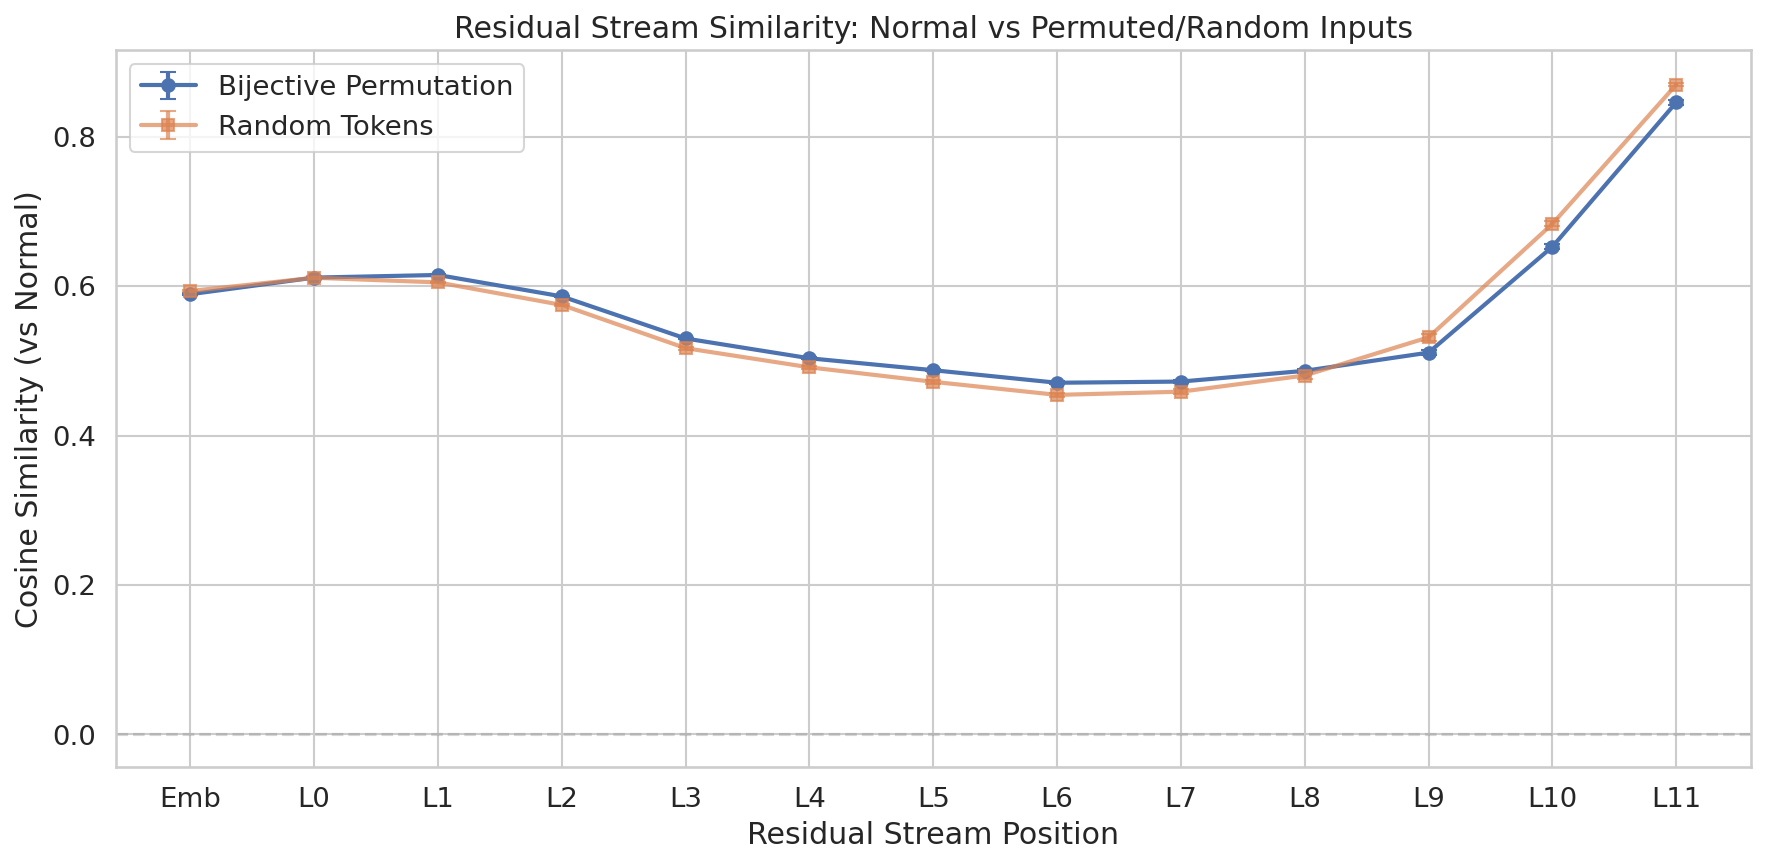
\includegraphics[width=\textwidth]{figures/layer_cosine_similarity.png}
        \caption{Cosine similarity (permuted vs.\ random baseline)}
        \label{fig:cosine_sim}
    \end{subfigure}
    \hfill
    \begin{subfigure}[b]{0.48\textwidth}
        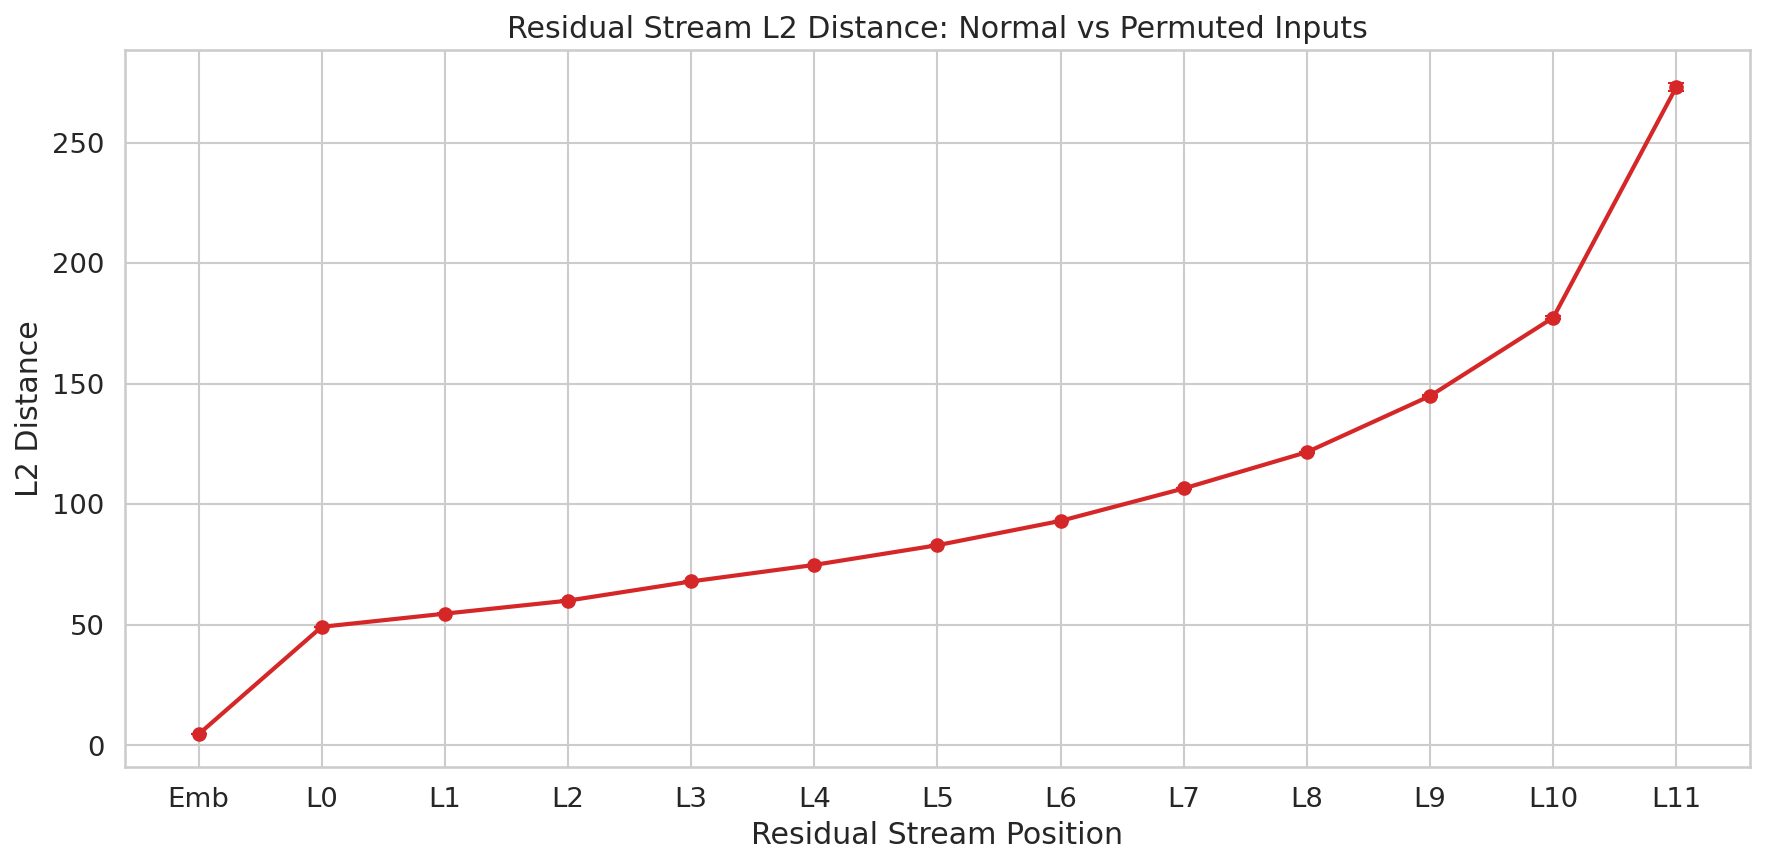
\includegraphics[width=\textwidth]{figures/l2_distance_layers.png}
        \caption{L2 distance between residual streams}
        \label{fig:l2_dist}
    \end{subfigure}
    \caption{Layer-wise comparison of normal vs.\ permuted residual streams. \captiona Cosine similarity follows a U-shaped trajectory, with the permuted condition (blue) nearly indistinguishable from random token replacement (orange). \captionb L2 distance grows monotonically from 4.6 (embedding) to 273.1 (layer 11), despite increasing cosine similarity at later layers. This dissociation indicates directional convergence at vastly different magnitudes.}
    \label{fig:layerwise}
\end{figure}

However, the L2 distance tells a different story (\figref{fig:l2_dist}): it grows monotonically from $4.60 \pm 0.01$ at the embedding layer to $273.14 \pm 1.64$ at layer 11---a 60$\times$ increase. This dissociation between cosine similarity and L2 distance means that while the residual stream vectors become more directionally aligned at later layers, they are simultaneously getting \emph{further apart} in absolute magnitude. \Tabref{tab:layerwise} provides the full numerical results.

\begin{table}[t]
    \centering
    \caption{Layer-wise cosine similarity and L2 distance between normal and permuted residual streams ($N=60$ samples, 256 tokens each). The U-shape in cosine similarity does not correspond to recovery---L2 distance increases monotonically.}
    \label{tab:layerwise}
    \resizebox{\textwidth}{!}{%
    \begin{tabular}{@{}lcccccccccccccc@{}}
        \toprule
        & Embed & L0 & L1 & L2 & L3 & L4 & L5 & L6 & L7 & L8 & L9 & L10 & L11 \\
        \midrule
        Cos.\ sim.\ & 0.589 & 0.612 & 0.615 & 0.586 & 0.530 & 0.504 & 0.488 & 0.471 & 0.472 & 0.487 & 0.511 & 0.653 & \textbf{0.846} \\
        {\scriptsize$\pm$ SE} & {\scriptsize .001} & {\scriptsize .001} & {\scriptsize .001} & {\scriptsize .001} & {\scriptsize .001} & {\scriptsize .001} & {\scriptsize .002} & {\scriptsize .002} & {\scriptsize .002} & {\scriptsize .003} & {\scriptsize .004} & {\scriptsize .004} & {\scriptsize .003} \\
        \midrule
        L2 dist.\ & 4.60 & 49.2 & 54.6 & 60.0 & 68.0 & 74.9 & 83.0 & 93.1 & 106.6 & 121.6 & 144.9 & 177.4 & \textbf{273.1} \\
        {\scriptsize$\pm$ SE} & {\scriptsize .01} & {\scriptsize .06} & {\scriptsize .09} & {\scriptsize .11} & {\scriptsize .11} & {\scriptsize .12} & {\scriptsize .11} & {\scriptsize .13} & {\scriptsize .17} & {\scriptsize .22} & {\scriptsize .38} & {\scriptsize .63} & {\scriptsize 1.64} \\
        \bottomrule
    \end{tabular}
    }
\end{table}

\subsection{Logit Lens Analysis}
\label{sec:logitlens}

The logit lens projects each layer's residual stream through the unembedding matrix to obtain next-token predictions. \Tabref{tab:logitlens} shows that the model's predictions under permutation \emph{never} match normal predictions---at any layer.

\begin{table}[t]
    \centering
    \caption{Logit lens analysis ($N=40$ samples). Top-1 match rate measures how often the permuted model's predicted token matches the normal model's. Perm-adjusted match applies $\invperm$ before comparison, testing whether the model predicts correctly ``in the permuted space.'' Both are near zero at all layers. KL divergence between prediction distributions is large throughout.}
    \label{tab:logitlens}
    \begin{tabular}{@{}lcccc@{}}
        \toprule
        Layer & Raw Top-1 Match & Perm-Adj.\ Match & $\KL$ (Raw) & $\KL$ (Adjusted) \\
        \midrule
        Embed & 0.03\% & 0.00\% & 22.56 & 22.78 \\
        L0 & 0.00\% & 0.00\% & 16.38 & 18.58 \\
        L5 & 0.04\% & 0.00\% & 13.83 & 17.06 \\
        L8 & 0.89\% & 0.00\% & 15.37 & 17.87 \\
        L11 & 0.55\% & \textbf{0.00\%} & 6.08 & 8.90 \\
        \bottomrule
    \end{tabular}
\end{table}

The raw top-1 match rate peaks at 0.89\% (layer 8) and is 0.55\% at the final layer---far below even random chance ($1/50{,}257 \approx 0.002\%$ per token, but with vocabulary frequency effects). More strikingly, the permutation-adjusted match rate is exactly 0.00\% at every layer: the model is not predicting ``the right token but in the permuted space.'' The model has no internal representation of the cipher.

The KL divergence between normal and permuted logit distributions decreases from 22.56 (embedding) to 6.08 (layer 11), mirroring the cosine similarity increase. This confirms that the distributions become \emph{more similar in shape} at later layers---but not similar enough to produce matching predictions.

\subsection{Context Length Effect}
\label{sec:context}

If the model were adapting to the permutation in context, we would expect cosine similarity to \emph{increase} with more tokens. \Figref{fig:context} shows the opposite: similarity consistently \emph{decreases} with token position at every layer.

\begin{figure}[t]
    \centering
    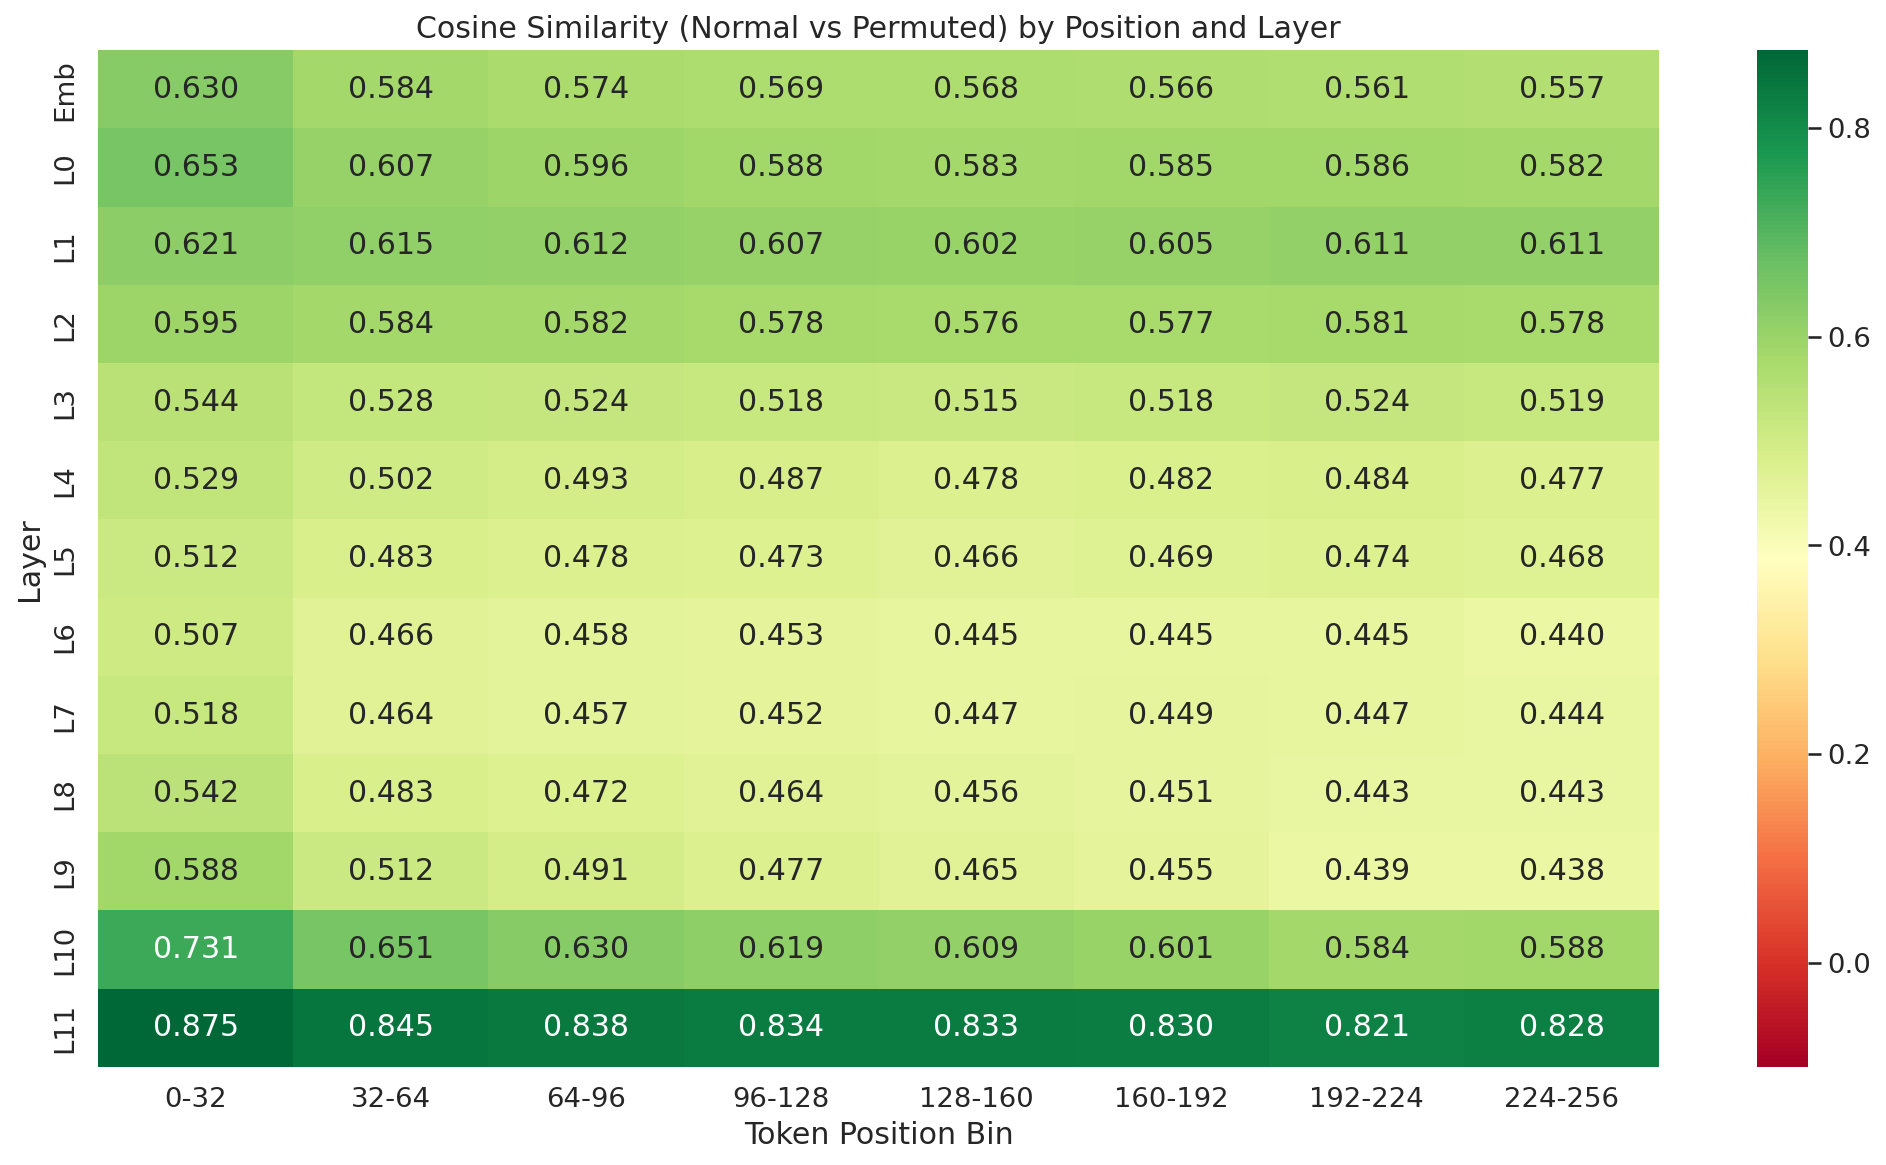
\includegraphics[width=0.65\textwidth]{figures/context_length_heatmap.png}
    \caption{Cosine similarity between normal and permuted residual streams as a function of token position (columns) and layer (rows). Similarity decreases with more context at all layers---the model gets \emph{worse}, not better, as it processes more permuted tokens. The Spearman correlation between position and similarity is $\rho = -0.98$ ($p < 0.001$).}
    \label{fig:context}
\end{figure}

\Tabref{tab:context} quantifies this pattern. At layer 11, similarity drops from 0.875 (positions 0--32) to 0.828 (positions 224--256). The Spearman rank correlations between token position and cosine similarity are strongly negative at all layers ($\rho = -0.76$ to $-0.98$, all $p < 0.03$). The model accumulates increasingly wrong contextual representations as it processes more permuted tokens.

\begin{table}[t]
    \centering
    \caption{Cosine similarity by token position bin and layer. Similarity decreases with more context at all layers, with statistically significant negative Spearman correlations.}
    \label{tab:context}
    \begin{tabular}{@{}lccccc@{}}
        \toprule
        Layer & Pos 0--32 & Pos 32--64 & Pos 96--128 & Pos 224--256 & Spearman $\rho$ \\
        \midrule
        Embed & 0.630 & 0.584 & 0.569 & 0.557 & $-0.98^{***}$ \\
        L6 & 0.507 & 0.466 & 0.453 & 0.440 & $-0.76^{*}$ \\
        L11 & 0.875 & 0.845 & 0.834 & 0.828 & $-0.93^{**}$ \\
        \bottomrule
        \multicolumn{6}{l}{\scriptsize $^{*}p<0.05$, $^{**}p<0.01$, $^{***}p<0.001$}
    \end{tabular}
\end{table}

\subsection{Norm Correlation and Attention Patterns}
\label{sec:norm}

\Figref{fig:norm} reveals a striking pattern in activation norms. The Pearson correlation between $\|\rs{\ell}_i\|$ and $\|\rsperm{\ell}_i\|$ across positions is nearly perfect through layers 2--10 ($r > 0.999$), then abruptly collapses at layer 11 ($r = 0.089 \pm 0.012$). This means that the model processes permuted input with nearly identical ``intensity profiles''---the same positions receive large activations---but the \emph{directions} of those activations are fundamentally different.

\begin{figure}[t]
    \centering
    \begin{subfigure}[b]{0.48\textwidth}
        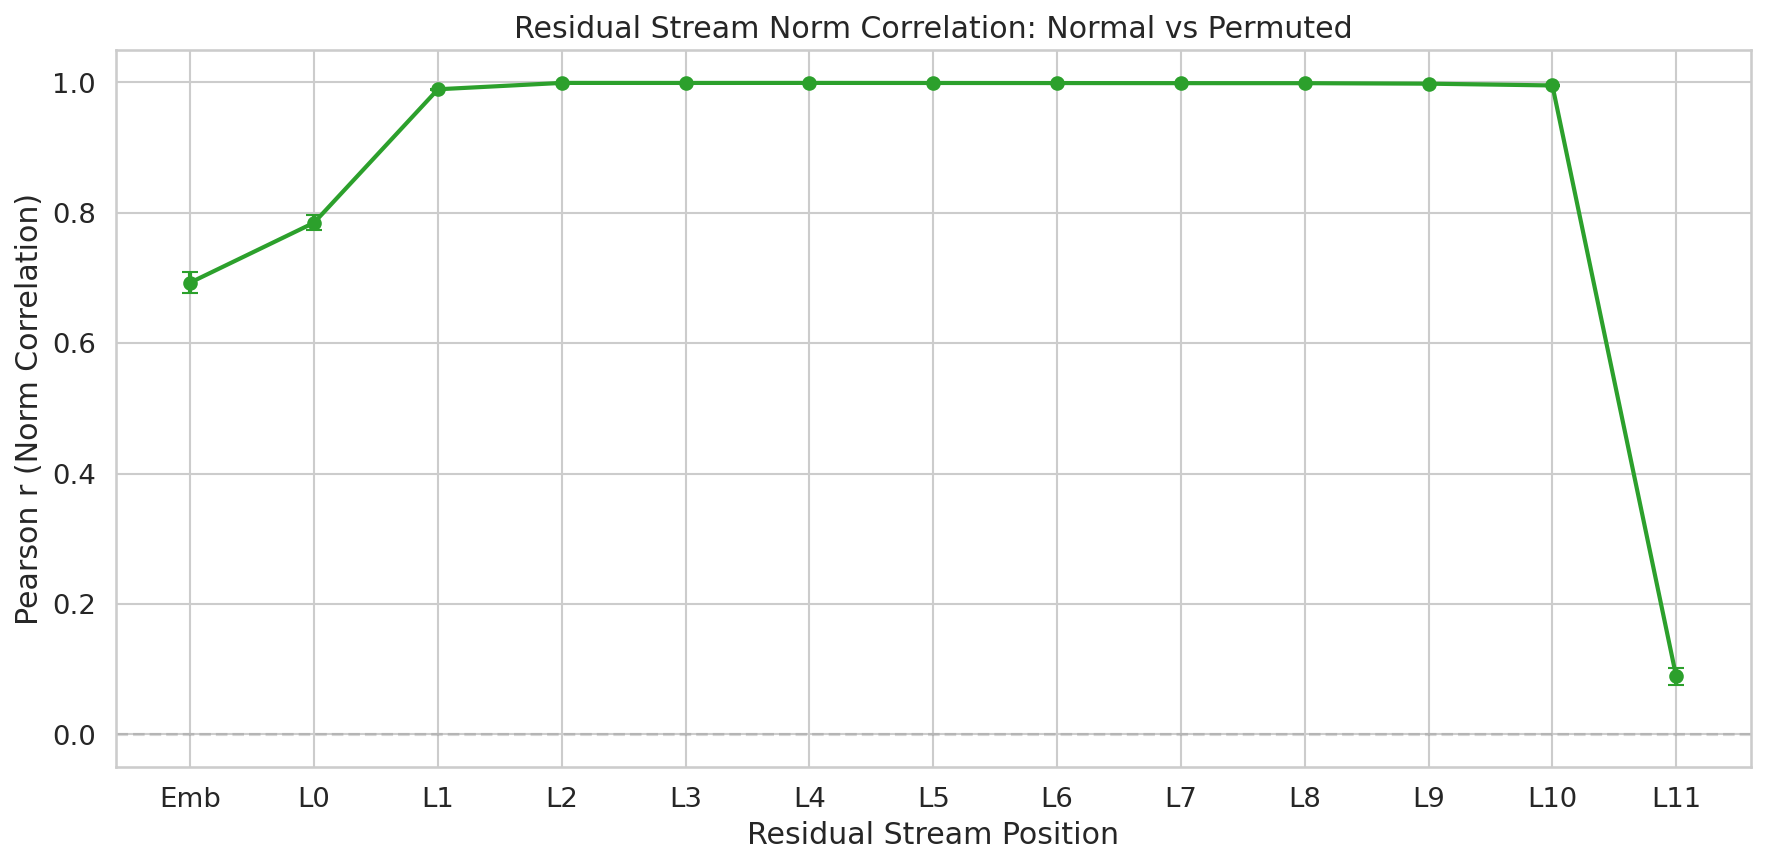
\includegraphics[width=\textwidth]{figures/norm_correlation_layers.png}
        \caption{Norm correlation across layers}
        \label{fig:norm}
    \end{subfigure}
    \hfill
    \begin{subfigure}[b]{0.48\textwidth}
        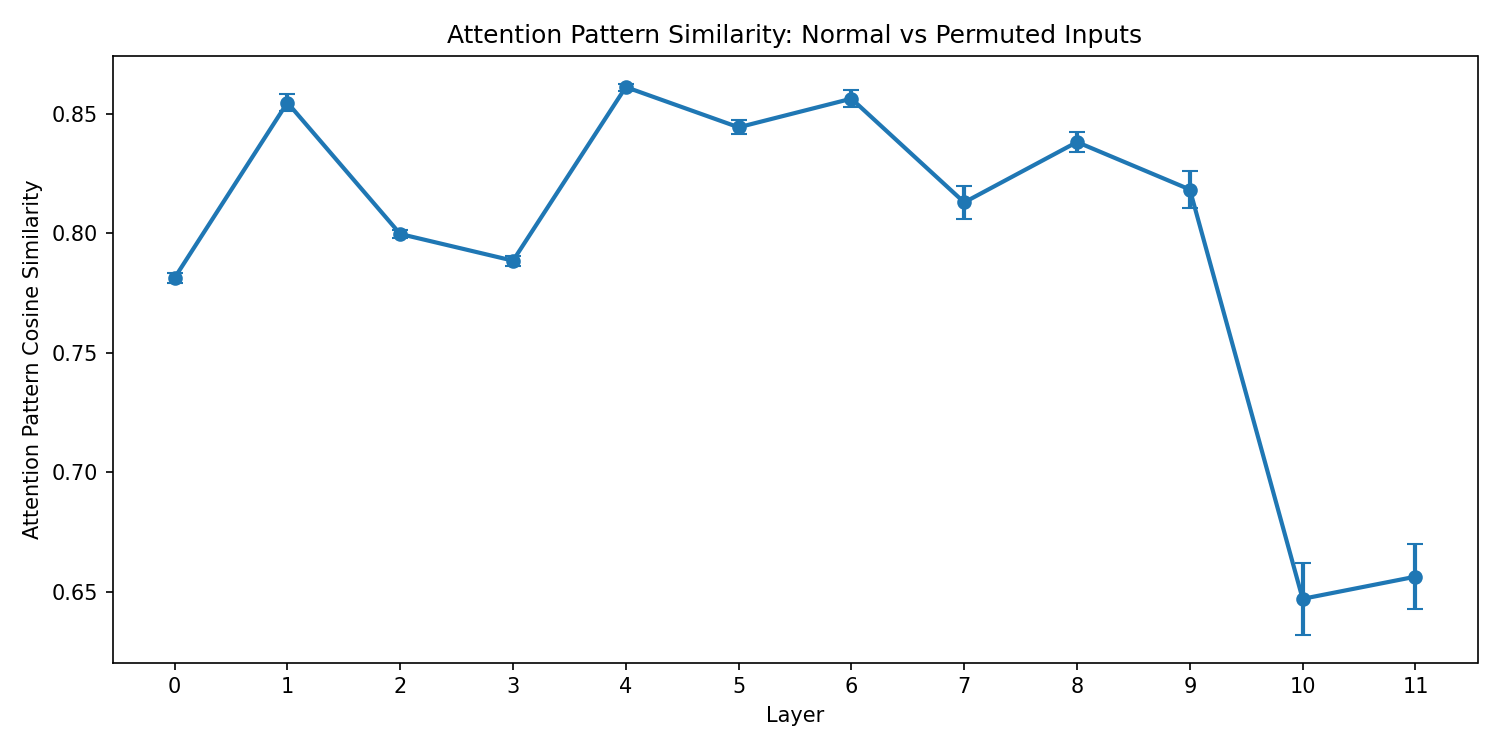
\includegraphics[width=\textwidth]{figures/attention_similarity.png}
        \caption{Attention pattern similarity}
        \label{fig:attention}
    \end{subfigure}
    \caption{\captiona Pearson correlation between activation norms under normal vs.\ permuted input. Norms are nearly perfectly correlated ($r > 0.999$) through layers 2--10, then collapse to $r = 0.089$ at layer 11. \captionb Attention pattern cosine similarity remains high (0.78--0.86) through layers 0--9, then drops to 0.65 at layers 10--11. The attention divergence at later layers coincides with the norm correlation collapse.}
    \label{fig:norm_attention}
\end{figure}

The norm correlation collapse at layer 11 coincides with a drop in attention pattern similarity (\figref{fig:attention}). Attention patterns remain fairly similar through layers 0--9 (mean cosine similarity 0.82, range 0.78--0.86), then drop to 0.65 at layers 10--11. Positional encoding and structural attention patterns are more robust to token identity changes than the content-dependent computations in the final layers.

\subsection{Random Baseline and Partial Permutation}
\label{sec:baselines}

\para{Random baseline.}
\Tabref{tab:random} compares cosine similarity when using a bijective permutation vs.\ random (non-bijective) token replacement. The differences are small ($|\Delta| < 0.03$) and inconsistent in sign. The bijective structure of the permutation provides no detectable advantage---a pre-trained model cannot exploit the fact that the mapping is one-to-one.

\begin{table}[t]
    \centering
    \caption{Cosine similarity: bijective permutation vs.\ random token replacement. Differences are small and inconsistent, indicating that the bijective structure provides no advantage. Statistical significance assessed via Wilcoxon signed-rank test.}
    \label{tab:random}
    \begin{tabular}{@{}lccc@{}}
        \toprule
        Layer & vs.\ Permuted & vs.\ Random & $\Delta$ \\
        \midrule
        L0 & 0.612 & 0.611 & $+0.001$ \\
        L5 & 0.488 & 0.472 & $+0.016$ \\
        L11 & 0.846 & 0.870 & $-0.024$ \\
        \bottomrule
    \end{tabular}
\end{table}

\para{Partial permutation.}
To understand how gracefully performance degrades, we vary the fraction of the vocabulary that is permuted from 0\% to 100\%. \Figref{fig:partial} shows that the U-shaped similarity curve is present at all permutation fractions, with degradation roughly proportional to the fraction permuted. Even 10\% permutation causes meaningful reduction in similarity, and the relationship is approximately linear.

\begin{figure}[t]
    \centering
    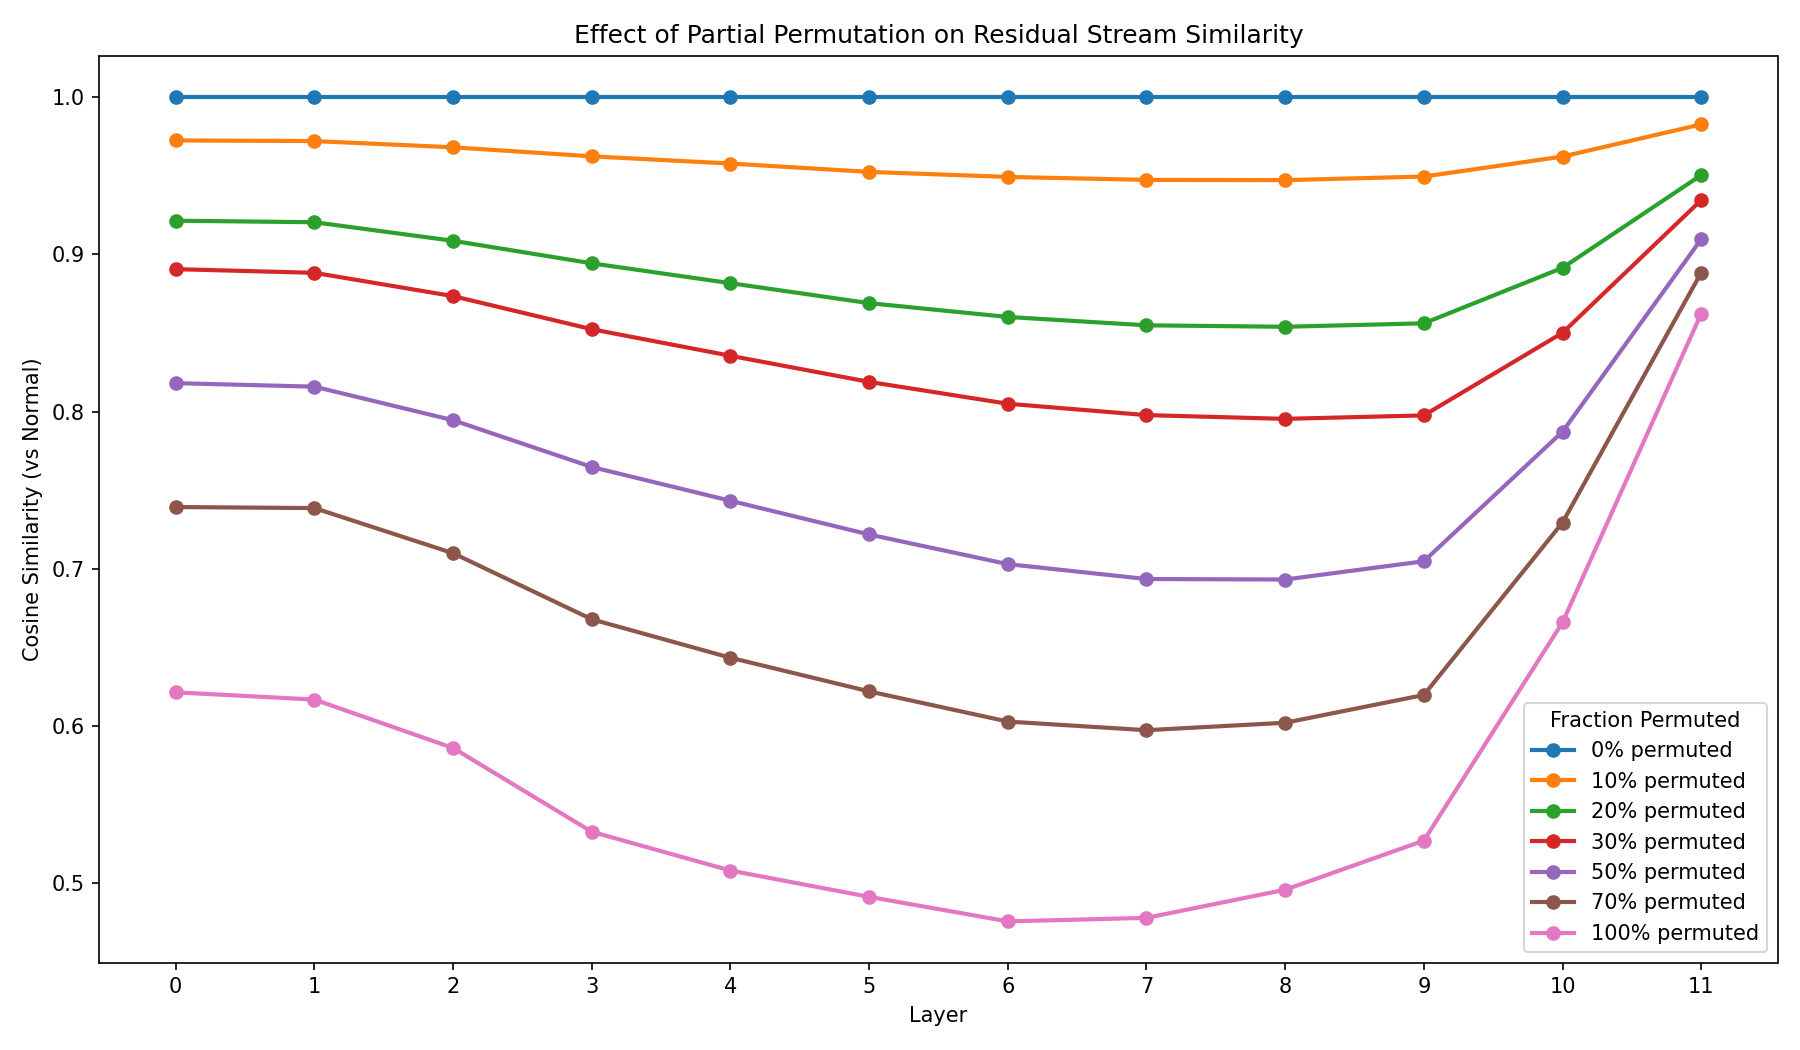
\includegraphics[width=0.65\textwidth]{figures/partial_permutation.png}
    \caption{Cosine similarity at selected layers as a function of the fraction of vocabulary permuted. The U-shape persists at all permutation fractions. Degradation is approximately linear with the fraction permuted---there is no sharp phase transition.}
    \label{fig:partial}
\end{figure}

\subsection{Perplexity}
\label{sec:perplexity}

The perplexity under normal processing is 47.5, consistent with GPT-2 Small's known performance on \wikitext. Under permutation (predicting the next \emph{permuted} token), perplexity rises to 109,989---a 2,315$\times$ increase. This confirms total failure at the task level, grounding the residual stream analysis in a concrete performance metric.
